\documentclass[tikz]{standalone}
%\usetikzlibrary{...}% tikz package already loaded by 'tikz' option
\usepackage{amsmath,amssymb}  % Pour les symboles mathématiques
\usepackage{lmodern}          % Utilisation de la police lmodern pour meilleure compatibilité SVG
\usetikzlibrary{matrix,positioning}
\usetikzlibrary{arrows.meta}

\begin{document}


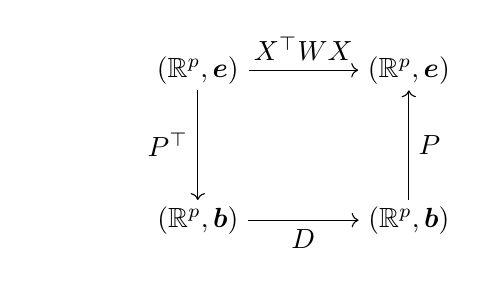
\begin{tikzpicture}
  \matrix (m) [matrix of math nodes, row sep=2em, column sep=4em, text height=1.5ex, text depth=0.25ex]
  {
    & (\mathbb{R}^p, \boldsymbol{e})  & (\mathbb{R}^p, \boldsymbol{e}) \\
    & & \\
    & (\mathbb{R}^p, \boldsymbol{b}) & (\mathbb{R}^p, \boldsymbol{b}) \\
  };

  % Flèches entre les cellules
  \path[->] (m-1-2) edge node[above] {$X^\top W X$} (m-1-3);
  \path[->] (m-1-2) edge node[left] {$P^\top$} (m-3-2);
  \path[->] (m-3-3) edge node[right] {$P$} (m-1-3);
  \path[->] (m-3-2) edge node[below] {$D$} (m-3-3);
  
  
\end{tikzpicture}

\end{document}